\section{Design}
\label{sec:design}

The original FlowQoS prototype was implemented on Raspberry Pi running OpenWrt Linux distribution with Openvswitch integration. However, since the aim of this paper is to validate the claims and results that demonstrate the need for FlowQoS-like systems rather than its deployment feasibility, we implement our solution within the virtual networking environment in end-host Linux distribution. Though such implementation can be still be easily moved to a dedicated device.

\begin{figure}[t]
\centering
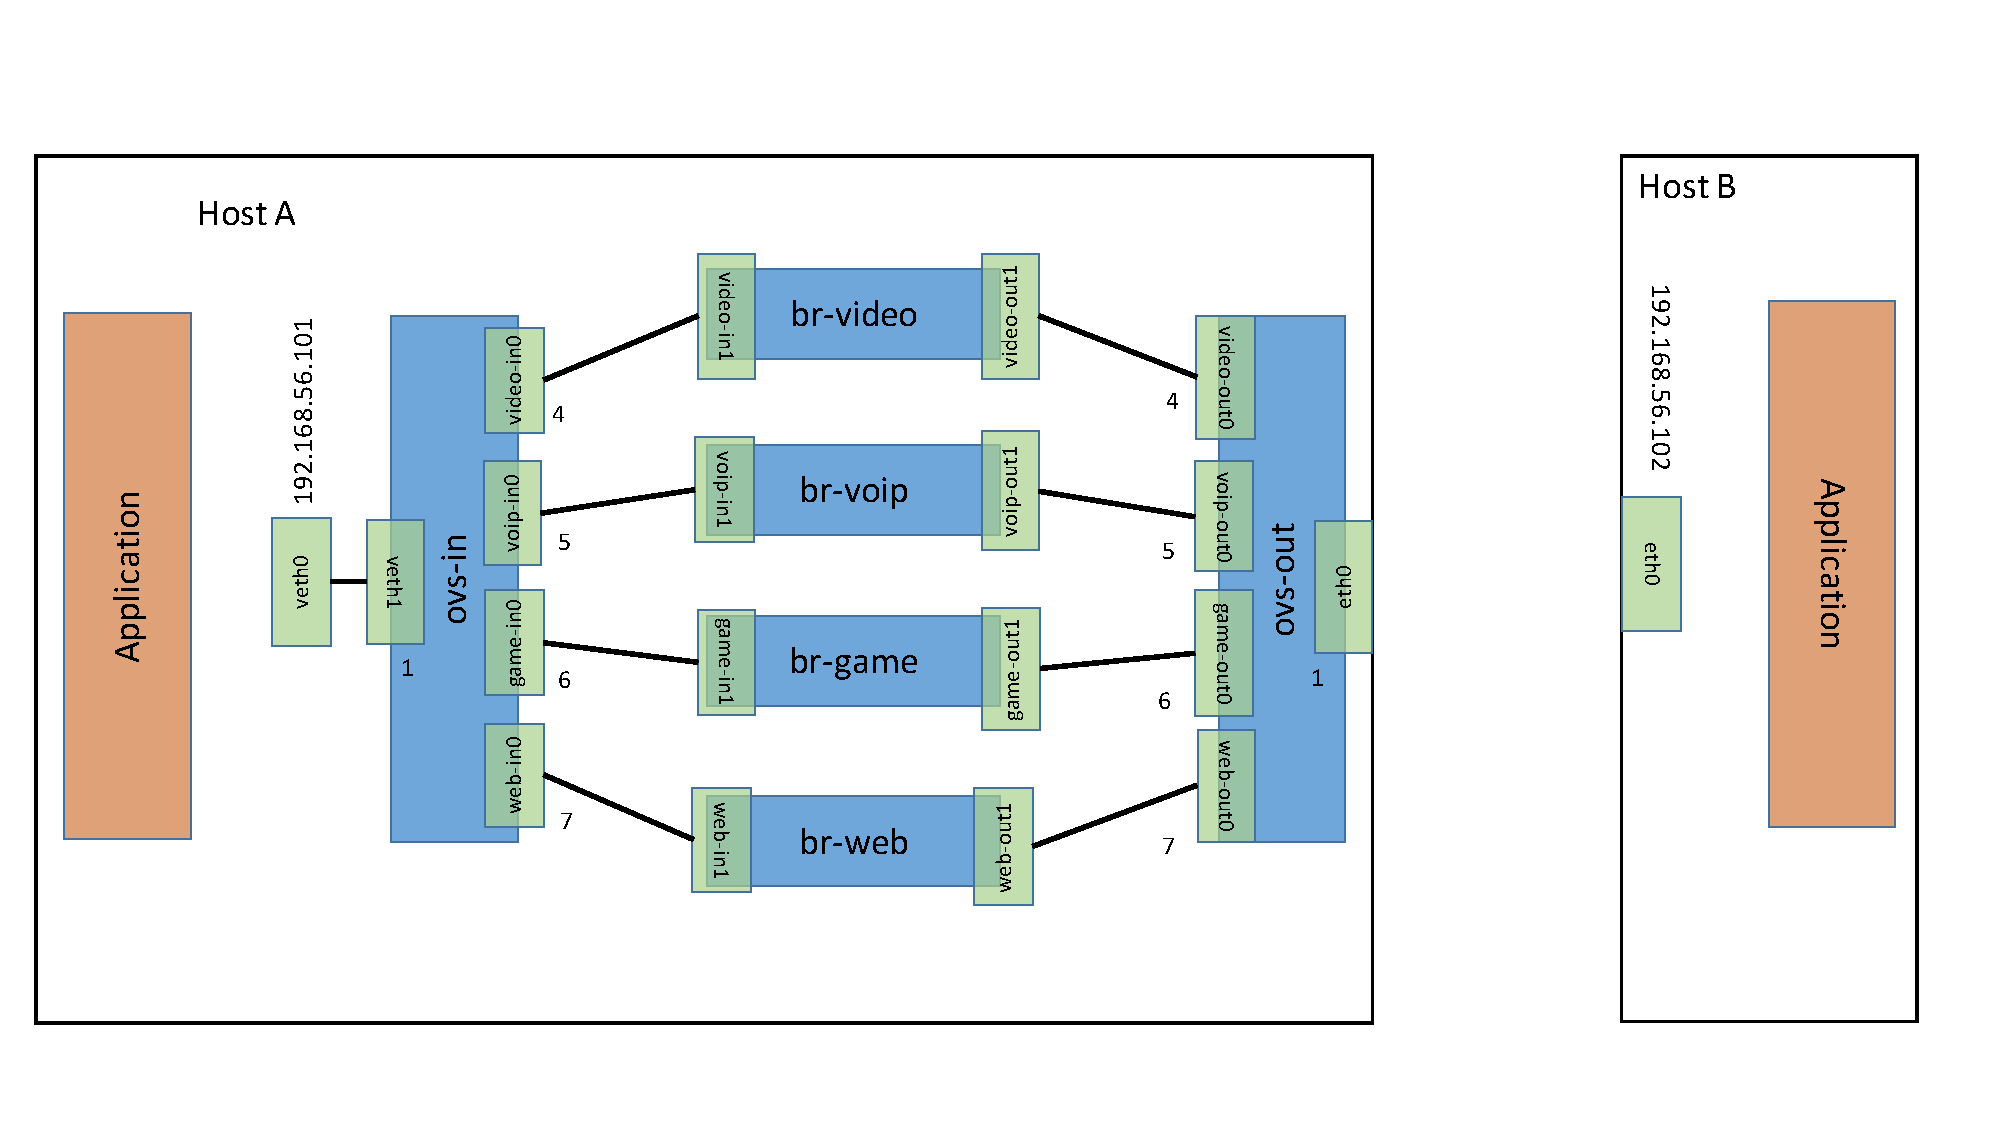
\includegraphics[width=0.9\linewidth]{architecture}
\caption{FlowQoS architecture.}
\label{fig:architecture}
\end{figure}

The FlowQoS's OVS-based architecture (~\fref{fig:architecture}) is comprised of dual-OVS topology with multiple paths between them passing through "dumb" forwarding bridges. Each path between the two OVSes (\texttt{ovs-in} and \texttt{ovs-out}) corresponds to a high-level traffic class to which the user or administrator wishes to classify any ingress (or egress) traffic to (or from) the end-host. Both \texttt{ovs-in} and \texttt{ovs-out} are configured to run in secure Openflow mode such that the OVS would accept Openflow commands from the Openflow controller when connected to it and in its absence it would not default to learning switch mode. This is required to prevent the runaway issue in learning switch network topologies with cycles. The physical interface (\texttt{eth0} in our case) connecting the end-host to the physical network is attached to \texttt{ovs-out}, whereas, the IP address for the end-host machine is moved from \texttt{eth0} to the virtual ethernet interface \texttt{veth0}. Such a setup ensures that any traffic from any application must traverse dual-OVS virtual topology before leaving the end-host and vice-versa for the incoming traffic. While the connecting bridges between \texttt{ovs-in} and \texttt{ovs-out} provide no functionality of their own, we use them solely for packet capture and debugging purposes.

In our implementation of HTB-based architecture, we combined \texttt{ovs-in} and \texttt{ovs-out} in ~\fref{fig:architecture} into one OVS and enable an HTB qdisc (queueing discipline) on \texttt{veth0} and \texttt{veth1}. To this qdisc, we added one parent class and four leaf classes each for one traffic type. The leaf classes are: \textbf{Video}, \textbf{VoIP}, \textbf{Gaming} and \textbf{Web}. To this, we added filters to classify the different traffic types and finally assign priorities to the each sub-class such that \textbf{Video} and \textbf{VoIP} get the highest priorities followed by \textbf{Web} traffic and finally the \textbf{Gaming} (unclassified) traffic gets the least priority.

We now discuss the two primary components of the FlowQoS controller module - namely, the Flow Classifier and the Rate Controller.

\subsection{Flow Classifier}
FlowQoS's classifier is comprised of two sub-modules - HTTP classifier and non-HTTP classifier. The reason for such initlal segregation is that modern HTTP applications no longer just carry textual web traffic but can include embedded components such as video players, advertisements, images etc. each generating traffic of different nature.
Therefore, identifying traffic to be HTTP is not sufficient and further analysis must be done to ascertain the type of traffic that the HTTP stream is actually carrying. Hence, any incoming packets from underlying Openflow layer are categorized HTTP (or HTTPS) based on the source or destination port being 80 (or 443).

With this goal in mind, FlowQoS was designed to inspect DNS queries that an HTTP application makes before it even sends or receives any HTTP traffic. The classifier uses a preconfigured list of DNS CNAME records to match a domain to its application type. The list is continuously updated based on the expiry time of DNS record. Hence, when an HTTP traffic has source or destination that matches the regular expression for that domain, it is classified based on the pre-identified traffic type.

On the other hand, for non-HTTP traffic, FlowQoS makes use of the \texttt{libprotoident} \cite{flow_web} library. The library requires certain additional information to be captured from the packets apart from the protocol type, source destination IP addresses and ports. Particularly, it uses the first 4 payload bytes and payload size for the first packet in either direction flows of a connection (or just one direction in case of unidirectional flows).

However, our initial exprimentation with applications we use to evaluate FlowQoS did not result in correct identification of the protocol due to multiple reasons such as unavailability of DNS resolution for locally hosted HTTP server and due to certain protocols (eg. Skype and Iperf TCP) not showing specific packet signature for classification by \texttt{libprotoident} library. Therefore, for our evaluation we fall back to the default port-based protocol identification technique.

\subsection{Rate Controller}
FlowQoS's rate controller hosts REST APIs to receive a bandwidth distribution from the user and generate a parsable JSON configuration file to used on the end-host to enforce rate limits on each kind of traffic.
Since, the primary focus of this paper is not to validate the accuracy of the flow classification, but rather the effectiveness of classification and rate limiting in improving application performance, we now evaluate the two different schemes of enforcing rate limits along with their pros and cons based on the evaluations with various traffic types in ~\xref{sec:evaluation}.
